\section{遷移問題への拡張}\label{chap:trans}

%%%%%%%%%%%%%%%%%%%%%%%%%%%%%%%%%%%%% 
\newcommand{\lw}[1]{\smash{\lower-8.ex\hbox{#1}}}
\begin{figure*}[htbp]
  %\renewcommand{\arraystretch}{0.9}
  \tabcolsep = 3mm  
  \centering
  \begin{tabular}{ccc}
    $t=0$ (スタート状態) & & $t=1$\\
    \scalebox{0.8}{%%%%%%%%%%%%%%%%%%%%%%%%%%%%%%%%%%%%%%%%%%%%%%%%%%
% 実行例(t=0) (第6章で使う)
%%%%%%%%%%%%%%%%%%%%%%%%%%%%%%%%%%%%%%%%%%%%%%%%%%

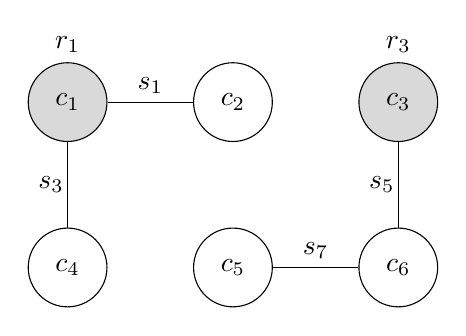
\begin{tikzpicture}[x=1.5cm,y=1.5cm,scale=0.7]

 % 設定
 \tikzset{root/.style={circle,draw=black,fill=gray!30,minimum size=1cm}}
 \tikzset{node/.style={circle,draw=black,minimum size=1cm}}
 
 % 補助線
 % \draw [help lines,blue,step=2cm] (-3,0) grid (3,-3);

 % 時間 %
 % \node[rectangle,draw=black] at (-3,1) {$t=0$};

 % root %
 \node[root] at (-2,0) (1){$c_1$};
 \node[above=0.5cm] at (1) {$r_1$};
 \node[root] at (2,0) (3){$c_3$};
 \node[above=0.5cm] at (3) {$r_3$};

 % node %
 \node[node] at (0,0) (2){$c_2$};
 \node[node] at (-2,-2) (4){$c_4$};
 \node[node] at (0,-2) (5){$c_5$};
 \node[node] at (2,-2) (6){$c_6$};

 % 繋がっていない辺は破線
 %\foreach \u / \v in {2/3, 2/5, 4/5}
 %\draw [dashed] (\u) -- (\v);
 % 繋がってる辺は実線
 \foreach \u / \v in {1/2, 1/4, 3/6, 5/6}
 \draw (\u) -- (\v);

 % スイッチ switch %
  \node at (-1,0.2) {$s_1$};
 % \node at (1,0.2) {$s_2$};
  \node at (-2.2,-1) {$s_3$};
 % \node at (-0.2,-1) {$s_4$};
  \node at (1.8,-1) {$s_5$};
 % \node at (-1,-1.8) {$s_6$};
  \node at (1,-1.8) {$s_7$};
 %

\end{tikzpicture}

%%%%%%%%%%%%%%%%%%%%%%%%%%%%%%%%%%%%%%%%%%%%%%%%%%%%%%%%%%
%%% Local Variables:
%%% mode: japanese-latex
%%% TeX-master: paper.tex
%%% End:
}
    & \lw{$\Rightarrow$} & 
    \scalebox{0.8}{%%%%%%%%%%%%%%%%%%%%%%%%%%%%%%%%%%%%%%%%%%%%%%%%%%
% 実行例(t=1) (第6章で使う)
%%%%%%%%%%%%%%%%%%%%%%%%%%%%%%%%%%%%%%%%%%%%%%%%%%

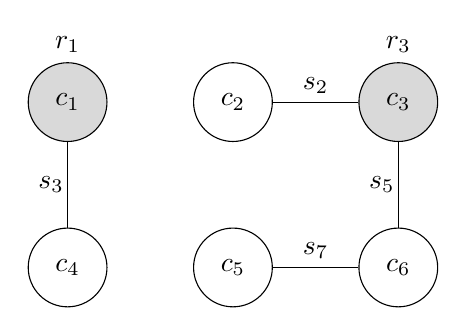
\begin{tikzpicture}[x=1.5cm,y=1.5cm,scale=0.7]

 % 設定
 \tikzset{root/.style={circle,draw=black,fill=gray!30,minimum size=1cm}}
 \tikzset{node/.style={circle,draw=black,minimum size=1cm}}
 
 % 補助線
 % \draw [help lines,blue,step=2cm] (-3,0) grid (3,-3);

 % 時間 %
 % \node[rectangle,draw=black] at (-3,1) {$t=1$};

 % root %
 \node[root] at (-2,0) (1){$c_1$};
 \node[above=0.5cm] at (1) {$r_1$};
 \node[root] at (2,0) (3){$c_3$};
 \node[above=0.5cm] at (3) {$r_3$};

 % node %
 \node[node] at (0,0) (2){$c_2$};
 \node[node] at (-2,-2) (4){$c_4$};
 \node[node] at (0,-2) (5){$c_5$};
 \node[node] at (2,-2) (6){$c_6$};

 % 繋がっていない辺は破線
 %\foreach \u / \v in {2/3, 2/5, 4/5}
 %\draw [dashed] (\u) -- (\v);
 % 繋がってる辺は実線
 \foreach \u / \v in {2/3, 1/4, 3/6, 5/6}
 \draw (\u) -- (\v);

 % スイッチ switch %
 % \node at (-1,0.2) {$s_1$};
 %
 \node at (1,0.2) {$s_2$};
 \node at (-2.2,-1) {$s_3$};
 % \node at (-0.2,-1) {$s_4$};
 \node at (1.8,-1) {$s_5$};
 % \node at (-1,-1.8) {$s_6$};
 \node at (1,-1.8) {$s_7$};
 %

\end{tikzpicture}

%%%%%%%%%%%%%%%%%%%%%%%%%%%%%%%%%%%%%%%%%%%%%%%%%%%%%%%%%%
%%% Local Variables:
%%% mode: japanese-latex
%%% TeX-master: paper.tex
%%% End:
}\\
    & & $\Downarrow$\\
    & & \\
    \scalebox{0.8}{%%%%%%%%%%%%%%%%%%%%%%%%%%%%%%%%%%%%%%%%%%%%%%%%%%
% 実行例(t=3) (第6章で使う)
%%%%%%%%%%%%%%%%%%%%%%%%%%%%%%%%%%%%%%%%%%%%%%%%%%
\begin{tikzpicture}[scale=0.6]

 % 設定
 \tikzset{node/.style={circle,draw=black,fill=white}}

 \definecolor{edge1}{RGB}{191,0,0}
 \definecolor{node1}{RGB}{249,200,200}
 \definecolor{edge3}{RGB}{38,38,134}
 \definecolor{node3}{RGB}{200,200,249}

 % 補助線
 % \draw [help lines,blue] (0,0) grid (20,6);

 % node %
 \node[circle, ultra thick, draw=edge1, fill=node1](out1){1};
 \node[node, fill=node3, right=of out1] (out2){2};
 \node[circle, ultra thick, draw=edge3,fill=node3, right=of out2](out3){3};
 \node[node, fill=node3, below=of out1] (out4){4};
 \node[node, fill=node3, below=of out2] (out5){5};
 \node[node, fill=node3, below=of out3] (out6){6};

 \foreach \u / \v in {}
 \draw [very thick, edge1] (\u) -- (\v);

 \foreach \u / \v in {out2/out3,out2/out5,out4/out5,out5/out6}
 \draw [very thick, edge3](\u) -- (\v);
\end{tikzpicture}

%%%%%%%%%%%%%%%%%%%%%%%%%%%%%%%%%%%%%%%%%%%%%%%%%%%%%%%%%%
%%% Local Variables:
%%% mode: japanese-latex
%%% TeX-master: paper.tex
%%% End:
}
    & \lw{$\Leftarrow$} &
    \scalebox{0.8}{%%%%%%%%%%%%%%%%%%%%%%%%%%%%%%%%%%%%%%%%%%%%%%%%%%
% 実行例(t=2) (第6章で使う)
%%%%%%%%%%%%%%%%%%%%%%%%%%%%%%%%%%%%%%%%%%%%%%%%%%

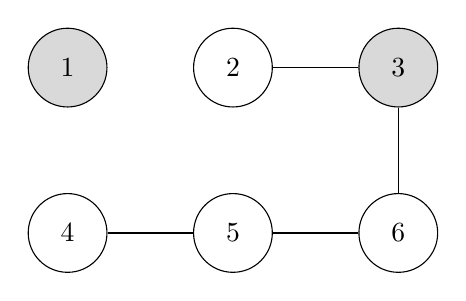
\begin{tikzpicture}[x=1.5cm,y=1.5cm,scale=0.7]

 % 設定
 \tikzset{root/.style={circle,draw=black,fill=gray!30,minimum size=1cm}}
 \tikzset{node/.style={circle,draw=black,minimum size=1cm}}
 
 % 補助線
 % \draw [help lines,blue,step=2cm] (-3,0) grid (3,-3);

 % 時間 %
 % \node[rectangle,draw=black] at (-3,1) {$t=2$};

 % root %
 \node[root] at (-2,0) (1){$1$};
% \node[above=0.5cm] at (1) {$r_1$};
 \node[root] at (2,0) (3){$3$};
 %\node[above=0.5cm] at (3) {$r_3$};

 % node %
 \node[node] at (0,0) (2){$2$};
 \node[node] at (-2,-2) (4){$4$};
 \node[node] at (0,-2) (5){$5$};
 \node[node] at (2,-2) (6){$6$};

 % 繋がっていない辺は破線
 %\foreach \u / \v in {2/3, 2/5, 4/5}
 %\draw [dashed] (\u) -- (\v);
 % 繋がってる辺は実線
 \foreach \u / \v in {2/3, 4/5, 3/6, 5/6}
 \draw (\u) -- (\v);

 % スイッチ switch %
 % \node at (-1,0.2) {$s_1$};
 % \node at (1,0.2) {$s_2$};
 % \node at (-2.2,-1) {$s_3$};
 % \node at (-0.2,-1) {$s_4$};
 % \node at (1.8,-1) {$s_5$};
 % \node at (-1,-1.8) {$s_6$};
 % \node at (1,-1.8) {$s_7$};
 %

\end{tikzpicture}

%%%%%%%%%%%%%%%%%%%%%%%%%%%%%%%%%%%%%%%%%%%%%%%%%%%%%%%%%%
%%% Local Variables:
%%% mode: japanese-latex
%%% TeX-master: paper.tex
%%% End:
}\\
    $t=3$ (ゴール状態) & & $t=2$
  \end{tabular}
  \caption{根付き全域森遷移問題 (遷移制約$d=2$) の解の一例}
  \label{fig:trans}
\end{figure*}
%%%%%%%%%%%%%%%%%%%%%%%%%%%%%%%%%%%%%

%%%%%%%%%%%%%%%%%%%%%%%%%%%%%%%%% 
\lstinputlisting[float=tb,caption={%
  全域森遷移問題のシングルショット符号化},%
captionpos=b,frame=single,label=code:roop,%
xrightmargin=1zw,% 
xleftmargin=1zw,% 
numbersep=5pt,%
numbers=left,%
breaklines=true,%
columns=fullflexible,keepspaces=true,%
basicstyle=\ttfamily\scriptsize]{code/trans-const.lp}
%%%%%%%%%%%%%%%%%%%%%%%%%%%%%%%%%

%%%%%%%%%%%%%%%%%%%%%%%%%%%%%%%%%
\lstinputlisting[float=tb,caption={%
  全域森遷移問題のマルチショット符号化},%
captionpos=b,frame=single,label=code:incmode,%
xrightmargin=1zw,% 
xleftmargin=1zw,% 
numbersep=5pt,%
numbers=left,%
breaklines=true,%
columns=fullflexible,keepspaces=true,%
basicstyle=\ttfamily\scriptsize]{code/dnet-trans.lp}
%%%%%%%%%%%%%%%%%%%%%%%%%%%%%%%%% 

配電網の構成制御における障害時の復旧予測への応用を狙いとし,
ある初期配電網構成(スタート状態)から目的配電網構成(ゴール状態)への
スイッチの切替手順を求める遷移問題を考える.
各ステップ$t$で切替可能なスイッチの個数を$d$個以下に制限し,
最短ステップ長での切替手順を求めることが目的である.

トポロジ制約のみを考える場合,この配電網の遷移問題は,
根付き全域森問題とその2つの実行可能解が与えられたとき,
ある解から他のもう一つの解へ根付き全域森の制約を満たしながら移る
``解の遷移問題''に帰着できる.
各ステップ$t$で変更可能な辺の数を$d$個以下に制限し(\textbf{遷移制約}),
最短ステップ長での変更手順を求めることが目的となる.
この遷移問題を根付き全域森遷移問題と呼ぶことにする.

図???\comment{???置換}の全域森問題とその2つの実行可能解から構成された
全域森遷移問題の解の一例を図~\ref{fig:trans}に示す
\comment{図中の数字は,$c_1$とか$s_1$の方がいい?}.
各ステップ$t$で変更可能な辺の数を$d=2$以下に制限している.
この解のステップ長は3であり,
スタート状態($t=0$)からゴール状態($t=3$)まで,
根付き全域森の制約を満たしながら遷移していることがわかる.

\textbf{シングルショット符号化.}
根付き全域森遷移問題のASP符号化をコード\ref{code:roop}に示す.
この符号化は,与えられた根付き全域森遷移問題に対して,ステップ長
\code{t}の解が存在するかを判定し,存在する場合はその解を返す論理プログ
ラムである.
根付き全域森問題の改良符号化(コード~\ref{code:srf2.lp})からの拡張点は
以下の通りである.
\begin{itemize}
\item 新しくステップを表すアトム\code{t(T)}を導入,
\item 改良符号化の各アトムにステップを表す項\code{T}を引数として追加,
\item スタート状態とステップ\code{0},ゴール状態とステップ\code{t}を対
  応させるルールを追加,
\item 遷移制約を表すルールを追加.
\end{itemize}
1行目の\code{t(0..t).}は,
\code{t(0).},
\code{t(1).},$\dots$
\code{t(t).}
に展開され,各ステップの識別子を表す.
定数\code{t}はスッテプ長を表す整数値であり,実行時に与えられる.

スタート状態はファクト\code{init_Forest/2}の集合で与えらる.
5行目のルールは,スタート状態とステップ\code{0}での
根付き全域森が一致することを強制する.
同様にして,
8行目のルールは,ゴール状態とステップ\code{t}での
根付き全域森が一致することを強制する.

遷移制約は30〜34行目のルールで表される.
\code{dist(X,Y,T)}は
ステップ\code{T-1}とステップ\code{T}の間で
辺\code{(X,Y)}に変化があったことを意味する.
34行目のルールは,各ステップ\code{T}において,
状態が変化した辺の数が\code{d}以下であることを保証する.

\textbf{マルチショット符号化.}
シングルショット符号化は,根付き全域森問題の改良符号化
(コード~\ref{code:srf2.lp})の自然な拡張になっている.
この符号化を用いて遷移問題を解くには,ステップ長\code{t}を増やしながら,
複数の問題を繰り返し解く必要がある.
しかし,各問題中の制約の大部分は共通であるため,ASP システムが同一の
探索空間を何度も調べることになり,求解効率が低下するという問題点がある.

この問題を解決するために,
ASPシステム{\clingo}のマルチショットASP解法を適用する.
この解法は,ASPシステムが同様の探索失敗を避けるために獲得した学習節を
(部分的に)保持することで,無駄な探索を行うことなく,制約を追加した論理
プログラムを連続的に解くことができる.そのため,求解性能の向上が期待できる.

ASPシステム{\clingo}のマルチショットASP解法ライブラリを用いた符号化を
コード~\ref{code:incmode}に示す.
この符号化は,\code{base},\code{step(t)},\code{check(t)}の3つのパー
トから構成される.
%
まず,\code{base}パートに,ステップ$t=0$で満たすべき制約を記述する.
ここでは,スタート状態とステップ\code{0}の対応を記述する(5行目).
%
次に,\code{step(t)}パートには,各ステップ\code{t}において満たすべき制
約を記述する.
ここでは,根付き全域森の制約と遷移制約を記述する(11〜37行目).
%
最後に,\code{check(t)}パートには,プログラムの終了条件を記述する.
ここでは,ゴール状態とステップ\code{t}の対応を記述する(43行目).
なお,\code{t}がインクリメントされると,一つ前の不要になった終了条件
は,\code{query(t)}の真偽を動的に操作することにより無効化される.

%%% Local Variables:
%%% mode: japanese-latex
%%% TeX-master: "paper"
%%% End:
